\chapter{Аналитический раздел}

В этом разделе будут представлены описание объектов, а также обоснован выбор алгоритмов, которые будут использован для ее визуализации.

\section{Описание объектов сцены}

Сцена состоит из источника света, цилиндра, жидкости, стержня и плоскости.

Источник света представляет собой материальную точку, пускающую лучи света во все стороны (если источник расположен в бесконечности, то лучи идут параллельно). Источником света в программе является вектор.
 
Цилиндр --- это тонкостенный прозрачный объект, в котором располагается два других объекта - жидкость, стержень.
  
Жидкость --- это объект, который тоже является прозрачным тонкостенным цилиндром.

Стержень --- это непрозрачный прямоугольный параллелепипед. Служит для того чтобы отобразить на экране преломление твердого тела в жидкости.

Плоскость --- это некая ограничивающая плоскость. Предполагается, что под такой плоскостью не расположено никаких объектов. Располагается на минимальной координате по оси У. 

\section{Обоснование выбора формы задания трехмерных моделей}

Отображением формы и размеров объектов являются модели. 
Обычно используются три формы задания моделей.

\begin{enumerate}
	\item Каркасная (проволочная) модель.
	
	Одна из простейших форм задания модели, так как мы храним информацию только о вершинах и ребрах нашего объекта. Недостаток данной модели состоит в том, что она не всегда точно передает представление о форме объекта.
	
	\item Поверхностная модель.
	
	Поверхностная модель объекта --- это оболочка объекта, пустая внутри. Такая информационная модель содержит данные только о внешних геометрических параметрах объекта. Такой тип модели часто используется в компьютерной графике. При этом могут использоваться различные типы поверхностей, ограничивающих объект, такие как полигональные модели, поверхности второго порядка и др.
	
	\item  Объемная (твердотельная) модель.
	
	При твердотельном моделировании учитывается еще материал, из которого изготовлен объект. То есть у нас имеется информация о том, с какой стороны поверхности расположен материал. Это делается с помощью указания направления внутренней нормали.
	
\end{enumerate}

При решении данной задачи будет использоваться объемная модель. Этот выбор обусловлен тем, что каркасные модели могут привести к неправильному восприятию формы объекта, а поверхностные модели не подходят, так как важен материал из которого сделаны объекты сцены.

\section{Задание объемных моделей}

После выбора модели, необходимо выбрать лучший способ представления объемной модели.

Аналитический способ --- этот способ задания модели характеризуется описанием модели объекта, которое доступно в неявной форме, то есть для получения визуальных характеристик необходимо дополнительно вычислять некоторую функцию, которая зависит от параметра.

Полигональной сеткой --- данный способ характеризуется совокупностью вершин, граней и ребер, которые определяют форму многогранного объекта в трехмерной компьютерной графике.

Стоит отметить, что одним из решающих факторов в выборе способа задания модели в данном проекте является скорость выполнения преобразований над объектами сцены.

При реализации программного продукта представлением является аналитический способ, так как все объекты в сцене являются простыми геометрическими фигурами.

\section{Выбор алгоритма удаления невидимых ребер и поверхностей}

Перед выбором алгоритма удаления невидимых ребер необходимо выделить несколько свойств, которыми должен обладать выбранный алгоритм, чтобы обеспечить оптимальную работу и реалистичное изображение, а именно:

\begin{itemize}
	\item	алгоритм должен использовать как можно меньше памяти;
	\item	алгоритм должен обладать небольшой относительно аналогичных алгоритмов трудоемкостью;
	\item	алгоритм должен выдавать реалистичное изображения.
\end{itemize}


\subsection{Алгоритм, использующий Z-буфер}
Суть данного алгоритма --- это использование двух буферов: буфера кадра, в котором хранятся атрибуты каждого пикселя, и Z-буфера, в котором хранится информация о координате Z для каждого пикселя.

Первоначально в Z-буфере находятся минимально возможные значения Z, а в буфере кадра располагаются пиксели, описывающие фон. Каждый многоугольник преобразуется в растровую форму и записывается в буфер кадра.

В процессе подсчета глубины нового пикселя, он сравнивается с тем значением, которое уже лежит в Z-буфере. Если новый пиксель расположен ближе к наблюдателю, чем предыдущий, то он заносится в буфер кадра и происходит корректировка Z-буфера \cite{zbufer}.

Для решения задачи вычисления глубины Z каждый многоугольник описывается уравнением $ax+by+cz+d=0$. При $c=0$ многоугольник для наблюдателя вырождается в линию. 

Для некоторой сканирующей строки y=const, поэтому имеется возможность рекуррентно высчитывать $z'$ для каждого $x'=x+dx$: $z' - z = - \frac{ax' + d}{c} + \frac{ax + d}{c} = \frac{a(x - x')}{c}$.

Получим $z' = z - \frac{a}{c}$, так как $x - x' = dx = 1$.

При этом стоит отметить, что для невыпуклых многогранников предварительно потребуется удалить не лицевые грани.

\subsubsection*{Преимущества}
\begin{itemize}
	\item простота реализации;
	\item оценка трудоемкости линейна.
\end{itemize}
\subsubsection*{Недостатки}
\begin{itemize}
	\item сложная реализация прозрачности;
	\item большой объем требуемой памяти.
\end{itemize}

%\subsubsection*{Вывод}
Данный алгоритм не подходит для решения поставленной задачи, так как требует большой объем памяти, и плохо работает с прозрачными объектами что не удовлетворяет требованиям. 



\subsection{Алгоритм Робертса}
Данный алгоритм работает в объектном пространстве, решая задачу только с выпуклыми телами.

Алгоритм выполняется в 3 этапа.

\textbf{Этап подготовки исходных данных}

На данном этапе должна быть задана информация о телах. Для каждого тела сцены должна быть сформирована матрица тела V. Размерность матрицы - $4*n$, где $n$ – количество граней тела.

Каждый столбец матрицы представляет собой четыре коэффициента уравнения плоскости  $ax+by+cz+d=0$, проходящей через очередную грань.

Таким образом, матрица тела будет представлена в следующем виде
\begin{equation}
	\label{eq:matr}
	V = \begin{pmatrix}
		a_{1} & a_{2} & \ldots & a_{n}\\
		b_{2} & b_{2} & \ldots & b_{n}\\
		c_{2} & c_{2} & \ddots & c_{n}\\
		d_{2} & d_{2} & \ldots & d_{n}
	\end{pmatrix}
\end{equation}

Матрица тела должна быть сформирована корректно, то есть любая точка, расположенная внутри тела, должна располагаться по положительную сторону от каждой грани тела. В случае, если для очередной грани условие не выполняется, соответствующий столбец матрицы надо умножить на -1. 

\textbf{Этап удаления рёбер, экранируемых самим телом}

На данном этапе рассматривается вектор взгляда $E=\{0, 0,-1, 0\}$.
Для определения невидимых граней достаточно умножить вектор $E$ на матрицу тела $V$. Отрицательные компоненты полученного вектора будут соответствовать невидимым граням.

\textbf{Этап удаления невидимых рёбер, экранируемых другими телами сцены}

На данном этапе для определения невидимых точек ребра требуется построить луч, соединяющий точку наблюдения с точкой на ребре. Точка будет невидимой, если луч на своём пути встречает в качестве преграды рассматриваемое тело \cite{roberts}.

\subsubsection*{Преимущества}
\begin{itemize}
	\item работа в объектном пространстве;
	\item высокая точность вычисления.
\end{itemize}

\subsubsection*{Недостатки}
\begin{itemize}
	\item рост сложности алгоритма --- квадрат числа объектов;
	\item тела сцены должны быть выпуклыми (усложнение алгоритма, так как нужна будет проверка на выпуклость);
	\item сложность реализации.
\end{itemize}

%\subsubsection*{Вывод}
Данный алгоритм не подходит для решения поставленной задачи из-за высокой сложности реализации как самого алгоритма, так и его модификаций, отсюда низкая производительность.


\subsection{Алгоритм художника}
Данный алгоритм работает аналогично тому, как художник рисует картину – то есть сначала рисуются дальние объекты, а затем более близкие. Наиболее распространенная реализация алгоритма --- сортировка по глубине, которая заключается в том, что произвольное множество граней сортируется по ближнему расстоянию от наблюдателя, а затем отсортированные грани выводятся на экран в порядке от самой дальней до самой ближней. Данный метод работает лучше для построения сцен, в которых отсутствуют пересекающиеся грани \cite{hudognik}. 

\subsubsection*{Преимущества}
\begin{itemize}
	\item	требование меньшей памяти, чем, например, алгоритм Z-буфера.
\end{itemize}

\subsubsection*{Недостатки}
\begin{itemize}
	\item	недостаточно высокая реалистичность изображения;
	\item	сложность реализации при пересечения граней на сцене.
\end{itemize}

%\subsubsection*{Вывод}
Данный алгоритм не отвечает главному требованию – реалистичности изображения. Также алгоритм художника отрисовывает все грани (в том числе и невидимые), на что тратится большая часть времени.


\subsection{Алгоритм Варнока}

Алгоритм Варнока \cite{varnok} является одним из примеров алгоритма, основанного на разбиении картинной плоскости на части, для каждой из которых исходная задача может быть решена достаточно просто.

Поскольку алгоритм Варнока нацелен на обработку картинки, он работает в пространстве изображения. В пространстве изображения рассматривается окно и решается вопрос о том, пусто ли оно, или его содержимое достаточно просто для визуализации. Если это не так, то окно разбивается на фрагменты до тех пор, пока содержимое фрагмента не станет достаточно простым для визуализации или его размер не достигнет требуемого предела разрешения.

Сравнивая область с проекциями всех граней, можно выделить случаи, когда изображение, получающееся в рассматриваемой области, определяется сразу:

\begin{itemize}
	\item	проекция ни одной грани не попадает в область;
	\item	проекция только одной грани содержится в области или пересекает область, то в этом случае проекции грани разбивают всю область на две части, одна из которых соответствует этой проекции;
	\item	существует грань, проекция которой полностью накрывает данную область, и эта грань расположена к картинной плоскости ближе, чем все остальные грани, проекции которых пересекают данную область, то в данном случае область соответствует этой грани.
\end{itemize}

Если ни один из рассмотренных трех случаев не имеет места, то снова разбиваем область на четыре равные части и проверяем выполнение этих условий для каждой из частей. Те части, для которых таким образом не удалось установить видимость, разбиваем снова и т. д.

\subsubsection*{Преимущества}
\begin{itemize}
	\item	меньшие затраты по времени в случае области, содержащий мало информации.
\end{itemize}


\subsubsection*{Недостатки}
\begin{itemize}
	\item	алгоритм работает только в пространстве изображений;
	\item	большие затраты по времени в случае области с высоким информационным содержимым.
\end{itemize}

%\subsubsection*{Вывод}
Данный алгоритм не отвечает требованию работы как в объектном пространстве, так и в пространстве изображений, а также возможны большие затраты по времени работы.


\subsection{Алгоритм обратной трассировки лучей}

Суть данного алгоритма состоит в том, что наблюдатель видит объект с помощью испускаемого света, который согласно законам оптики доходит до наблюдателя некоторым путем. Отслеживать пути лучей от источника к наблюдателю неэффективно с точки зрения вычислений, поэтому наилучшим способом будет отслеживание путей в обратном направлении, то есть от наблюдателя к объекту.

Предполагается, что сцена уже преобразована в пространство изображения, а точка, в которой находится наблюдатель, находится в бесконечности на положительной полуоси Z, и поэтому световые лучи параллельны этой же оси. При этом каждый луч проходит через центр пикселя растра до сцены. Траектория каждого луча отслеживается для определения факта пересечения определенных объектов сцены с этими лучами. При этом необходимо проверить пересечение каждого объекта сцены с каждым лучом, а пересечение с $Z_{min}$  представляет видимую поверхность для данного пикселя \cite{raytrace}.
 

\subsubsection*{Преимущества}
\begin{itemize}
	\item	высокая реалистичность синтезируемого изображения;
	\item	работа с поверхностями в математической форме;
	\item	вычислительная сложность слабо зависит от сложности сцены.
\end{itemize}

\subsubsection*{Недостатки}
\begin{itemize}
	\item	производительность.
\end{itemize}

%\subsubsection*{Вывод}
Данный алгоритм подходит для реализации реалистичных прозрачных объектов


\subsection{Вывод}

Для удаления невидимых линий выбран алгоритм обратной трассировки лучей. Данный алгоритм позволит добиться максимальной реалистичности и даст возможность смоделировать распространение света в пространстве, учитывая законы геометрической оптики. Также этот алгоритм позволяет строить качественные тени с учетом большого числа источников, и в данном алгоритме удобнее всего реализовывать прозрачные и матовые объекты, что позволит получить достаточно реалистичное изображение. Стоит отметить тот факт, что алгоритм трассировки лучей не требователен к памяти, в отличие, например, от алгоритма Z-буфера.



\section{Анализ и выбор модели освещения}

Физические модели материалов стараются аппроксимировать свойства некоторого реального материала. Такие модели учитывают особенности поверхности материала или же поведение частиц материала.

Эмпирические модели материалов устроены иначе, чем физически обоснованные. Данные модели подразумевают некий набор параметров, которые не имеют физической интерпретации, но которые позволяют с помощью подбора получить нужный вид модели.

В данной работе следует делать выбор из эмпирических моделей, а конкретно из модели Ламберта и модели Фонга.

\subsection{Модель Ламберта}

Модель Ламберта \cite{lamber_fong} моделирует идеальное диффузное освещение, то есть свет при попадании на поверхность рассеивается равномерно во все стороны. При такой модели освещения учитывается только ориентация поверхности ($N$) и направление источника света ($L$). Иллюстрация данной модели представлена на рисунке \ref{img:mod_lam}.

\begin{figure}[ht!]
	\begin{center}
		\captionsetup{singlelinecheck = false, justification=centerfirst}
		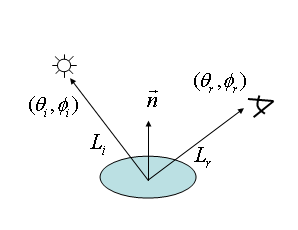
\includegraphics[scale=0.8]{assets/mod_lam.png}
		\caption{Модель освещения Ламберта}
		\label{img:mod_lam}
	\end{center}
	
	
\end{figure}

Эта модель является одной из самых простых моделей освещения и очень часто используется в комбинации с другими моделями.

\subsection{Модель Фонга}

Это классическая модель освещения. Модель представляет собой комбинацию диффузной и зеркальной составляющих. Работает модель таким образом, что кроме равномерного освещения на материале могут появляться блики. Местонахождение блика на объекте определяется из закона равенства углов падения и отражения. Чем ближе наблюдатель к углам отражения, тем выше яркость соответствующей точки \cite{lamber_fong}.

\begin{figure}[ht!]
	\begin{center}
		\captionsetup{singlelinecheck = false, justification=centerfirst}
		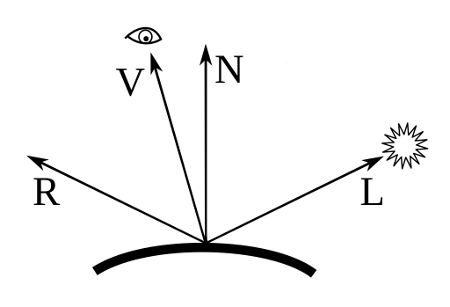
\includegraphics[scale=0.8]{assets/mod_fong.png}
		\caption{Модель освещения Фонга}
		\label{img:mod_fong}
	\end{center}
	
\end{figure}


Падающий и отраженный лучи лежат в одной плоскости с нормалью к отражающей поверхности в точке падения (рисунок \ref{img:mod_fong}). Нормаль делит угол между лучами на две равные части. $L$ – направление источника света, $R$ – направление отраженного луча, $V$ – направление на наблюдателя.

\subsection{Вывод}
Для освещения выбрана модель Фонга, так как изображение должно быть наиболее приближенным к реальности.

\section{Вывод}
В данном разделе был проведен анализ алгоритмов удаления невидимых линий и модели освещения, которые возможно использовать для решения поставленных задач. В качестве ключевого алгоритма выбран алгоритм обратной трассировки лучей, который будет реализован в рамках данного курсового проекта.

